\section{系统分析与设计}

系统分析TIMKE协议的设计目标、核心要求与实现方案能为协议接下来的实现工作提供方向。最终的实现在保持协议安全属性的同时,还应该拥有合适的计算和通信效率,并能在实际环境中部署。为确保工作的正常开展,在设计初期需要确立整体实现架构与开发技术。本节将讨论TIMKE协议的相关设计,介绍整体实现路线与技术决策。

\subsection{TIMKE协议的目标与要求}
\label{appendix:timke_protocol_goals}
实现密钥交换协议需要考虑安全性、功能性、性能及实现等多方面,TIMKE的实现有如下安全目标与功能要求:

\textbf{后量子安全.} 如今的加密协议实例都应该保证后量子安全,先前部署的加密实例也在向后量子安全的方向迁移。Shor算法在理论上能够破解基于离散对数和大整数分解问题的传统密码原语,随着量子计算的不断发展,未来会对现代的网络环境构成重大威胁。TIMKE协议采用后量子安全算法作为核心构件,采用的KEM基于格原语构造。格密码安全主要依赖于最短向量问题和最近向量问题等计算性难题,即使在量子计算模型下仍未发现高效的解法。

\textbf{紧致安全.} 传统密钥交换协议证明时通常包含与用户数量(n)和会话数量(n')相关的损失因子,导致协议的实际安全强度会因部署规模的扩大而降低。典型的安全损失可能是O(n*n')级别,在拥有数百万用户和会话的大规模系统中,协议部署需要使用远高于理论安全级别的参数才能维持安全,计算和通信开销较大。TIMKE协议利用多用户多挑战安全的KEM证明了紧致安全\cite{timke_2024},在大规模部署环境中无需过度增加参数大小。

\textbf{多阶段安全.} 现代网络协议(如TLS 1.3\cite{tls13_2018})大多采用多阶段密钥派生机制,不同阶段的密钥具有不同的安全属性和应用场景。TIMKE协议执行主要划分为两个阶段,第一阶段基于服务器长期密钥建立初始安全通道,并支持0-RTT数据传输;第二阶段引入客户端临时密钥对,提供更强的安全保障。第二阶段提供弱前向安全性,即使服务器的长期密钥泄露,若攻击者对第二阶段仅采取被动攻击,第二阶段的会话密钥仍能保持安全,为用户提供额外的安全保障。

\textbf{单边认证安全.} 实际网络环境如访问互联网等场景,通常只需对服务器进行身份认证,而客户端的身份认证可以在应用层通过账号密码等机制单独处理。TIMKE协议专注于单边认证模型,并保证:1) 在被动攻击场景中,服务器能够确认会话密钥仅与持有正确客户端密钥的实体共享;2) 在主动攻击场景中,客户端能够确认会话密钥仅与持有已验证服务器私钥的实体共享。这种设计在保持协议结构简洁的同时,满足了大多数客户端——服务器交互场景的安全需求,并为有需要的应用提供了在上层协议中实现完整双向认证的灵活性。

\textbf{双阶段密钥派生.} 现代网络协议(如TLS 1.3和QUIC)通常采用多阶段密钥派生机制,以支持不同的安全需求和功能特性。TIMKE协议采用两阶段架构:第一阶段基于OW-ChCCA安全的KEM实现,使用服务器的长期公钥构件安全信道,支持0-RTT数据传输以提供快速响应;第二阶段基于单向明文可检测攻击(One-Wayness under Plaintext-Checking Attacks, OW-PCA)安全的KEM实现,引入客户端临时密钥对,建立具有弱前向安全性的主会话密钥,用于后续的报文通信。协议设计在保持清晰结构的同时还提供了分层的安全保障,允许用户按需选择加密参数,未来能在一定程度上与 QUIC 协议兼容。
    
\textbf{0-RTT数据传输.} 网络延迟关乎用户日常使用,过高的延迟网络环境会影响用户体验,如网页浏览、实时通信等场景。传统的网络协议在握手环节通常需要多次往返才能建立安全通道,而TIMKE协议支持0-RTT(零往返时间)数据传输,允许客户端在有服务器预共享公钥的情况下直接发送加密的应用数据,无需等待服务器首轮响应,提升用户体验和应用响应速度。

\textbf{通用构造.} 密码学算法和安全威胁是持续发展变化的,协议设计需要拥有足够的灵活性以具备一定抗性。TIMKE协议采用通用构造方式,将核心密码原语(如KEM)抽象为接口,允许灵活嵌入不同的后量子安全KEM算法,以支持未来适配新的后量子密码标准或加密算法。当前的协议实现支持多种KEM的集成(如ML-KEM、OW-ChCCA KEM),允许自选安全级别,自定义各阶段的KEM实例,延长协议的生命周期,降低升级和维护成本。

\subsection{协议实现方案}

TIMKE协议建立在一系列密码学组件之上,共同构成协议的安全基础。实现采用模块化设计,将各组件封装为独立接口,分离功能模块,支持灵活配置。

\subsubsection{核心密码组件}
\textbf{KEM\textsubscript{1}.} 具有OW-ChCCA安全性的密钥封装机制,用于构建服务器长期密钥对。KEM\textsubscript{1}需要满足$(1-\delta_1)$-正确性(其中$\delta_1 = negl(\lambda)$为可忽略函数),具有$\gamma_1$比特的密文熵和$\mu_1$比特的公钥熵。OW-ChCCA安全性是一种独特的密钥封装安全定义,允许敌手查询"可检测"的解封装预言机,同时保持紧致安全。

\textbf{KEM\textsubscript{2}.} 具有$(N,\mu)$-OW-PCA安全性的密钥封装机制,用于客户端生成临时密钥对。KEM\textsubscript{2}需要满足$(1-\delta_2)$-正确性(其中$\delta_2 = negl(\lambda)$为可忽略函数),具有$\gamma_2$比特的密文熵和$\mu_2$比特的公钥熵。OW-PCA安全性比传统IND-CCA2安全性要求更低,但在TIMKE协议的整体结构中足以提供必要的安全保证,同时降低计算开销。理论上,任何IND-CCA2安全的KEM都满足OW-PCA安全性,实现中使用后量子安全KEM作为KEM\textsubscript{2},简化协议的实现和部署。

\textbf{哈希函数H\textsubscript{1}和H\textsubscript{2}.} 选择NIST标准推荐的SHA3-512作为哈希函数,分别用于从KEM共享密钥派生临时会话密钥和主会话密钥。在安全分析中,它们被建模为随机预言机(Random Oracle Model, ROM),提供理想的安全属性。H\textsubscript{1}: $\{0,1\}^* \rightarrow$ SK映射到临时会话密钥空间;H\textsubscript{2}: $\{0,1\}^* \rightarrow$ SK'映射到主会话密钥空间,确保会话密钥的唯一性和不可预测性,同时捕获协议状态的完整上下文。

\textbf{对称加密方案D = (Enc, Dec).} 用于保护协议中传输的应用数据,需要满足标准的语义安全。Enc函数使用会话密钥加密明文消息,Dec函数使用相同的会话密钥解密。实现中使用AES-GCM作为对称加密算法,该算法同时还提供保密性和完整性保护,是许多现代网络协议的可选方案之一。

TIMKE协议的安全证明将整体安全性归约到这些基础组件的安全性,特别是两个KEM的安全性,因此这些组件的安全性会直接影响协议的整体安全。

\subsubsection{协议工作流程}
TIMKE协议的工作流程如图\ref{fig:protocol-flow}所示,分为预共享阶段、第一阶段和第二阶段三个部分,符合现代密钥交换协议的通用模式,也支持0-RTT数据传输等高级功能。

在预共享阶段,服务器生成长期密钥对并将公钥分发给客户端,与TLS中证书的分发相似,可通过公钥基础设施或其他可信渠道实现。第一阶段,客户端使用服务器公钥封装共享密钥,派生出临时会话密钥,并可选地发送0-RTT加密数据。服务器收到请求后,解封装共享密钥,派生相同的临时会话密钥,并处理0-RTT数据。在第二阶段,服务器使用客户端临时公钥封装另一个共享密钥,双方共同派生主会话密钥,建立更安全的通信通道。在保持协议简洁性的同时,提供了分层的安全保障和功能支持。
\begin{figure}[ht]
    \centering
    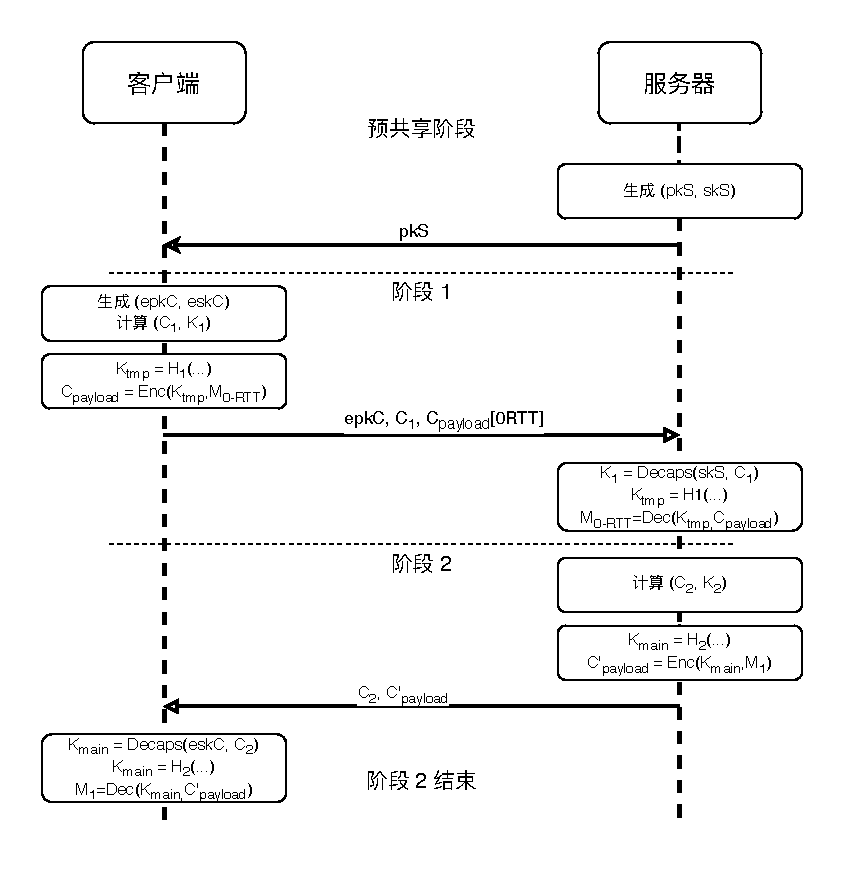
\includegraphics[width=0.75\textwidth]{doc/graph/protocol.drawio.pdf}
    \caption{TIMKE协议流程图}
    \label{fig:protocol-flow}
\end{figure}

\subsubsection{实现路线与技术决策}

现实中缺少OW-ChCCA安全KEM的实现方案,需基于论文\cite{pan_lattice-based_2023}中的理论构造设计并实现,详细内容见第\ref{chap:owchccakem}章。参考现代网络协议(如TLS 1.3和QUIC)的设计思路确定协议整体架构,如模块化结构和状态管理机制,使TIMKE协议能够与现有安全基础设施更好地集成,降低部署和使用的门槛。在评估现有资源和技术挑战后,制定出以下实现路线。

首先,开发并测试核心密码组件,包括OW-ChCCA KEM和密钥派生函数。之后实现TIMKE协议,包括状态管理和消息处理逻辑,再构建支持0-RTT数据传输的客户端-服务器演示系统。最后,对实现结果进行全面的性能测试,验证协议的功能正确性,对不同KEM组合在各种操作环境下的性能进行系统分析。

\subsection{开发环境}
所有代码的编写与运行环境概述如下,
\begin{itemize}
  \item 操作系统:MacOS Sequoia 15
  \item 芯片:Apple M1 Pro(8核,6性能/2能效)
  \item 内存:16GB
  \item 开发工具:Visual Studio Code / Goland / Bash / iTerm2
\end{itemize}

选择Go语言(Golang)作为主要实现语言,基于多方面考虑,
\begin{itemize}
  \item Go标准库提供了完善的密码学支持,包括各种哈希函数、对称加密算法和随机数生成器
  \item Go的静态类型系统和内存安全特性降低了安全漏洞的风险,适合密码协议的实现
  \item Go的跨平台兼容性优秀,同一套代码可以在不同操作系统和处理器架构上运行,简化部署
  \item Go的编译速度快,开发-测试循环高效,提高了实现过程中的迭代速度
  \item Go拥有强大的并发处理能力,适合实现如OW-ChCCA KEM中大矩阵运算等计算密集型任务
\end{itemize}

虽然本实现选择Go语言作为主要开发语言,但协议设计和关键算法原理并不依赖于特定编程语言。理论上,TIMKE协议可以使用多种高级编程语言实现:

\begin{itemize}
  \item \textbf{C/C++}:作为更底层的编程语言,提供细致的内存管理,能对执行的效率进行把控,适合资源受限设备和高性能计算环境。对于OW-ChCCA KEM中的大矩阵运算,使用OpenMP框架或SIMD指令集可达到更高的计算吞吐量。
  
  \item \textbf{Rust}:在提供内存安全保证同时保持接近C++的性能,适合安全关键型应用。Rust的所有权模型在实现环节帮助开发者防止常见的内存安全漏洞。
  
  \item \textbf{Python}:虽然解释型语言在密码协议的性能上有劣势,但结合NumPy等高性能计算库以及丰富的生态环节,适用于原型设计和演示。
\end{itemize}

使用Bash脚本语言开发了自动化测试套件和演示脚本,简化了测试过程和系统展示。

为促进开源协作和学术交流,所有代码和相关文档已开源在GitHub平台:

1. \href{https://github.com/MingLLuo/OW-ChCCA-KEM}{OW-ChCCA-KEM实现}:\url{{https://github.com/MingLLuo/OW-ChCCA-KEM}}

2. \href{https://github.com/MingLLuo/TIMKE/}{TIMKE实现}:\url{https://github.com/MingLLuo/TIMKE/}